\chapter{Sistema propuesto: teoría y simulaciones}

\begin{figure}[t]
\centering
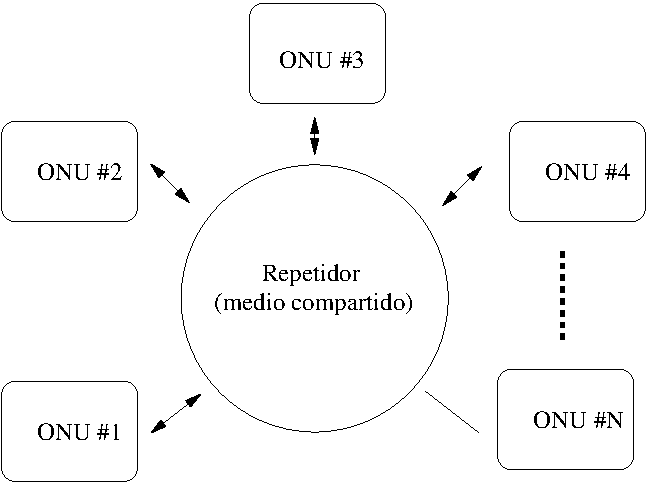
\includegraphics[width=4in]{graphs/hub}
\caption{Estructura de alto nivel del sistema propuesto, donde un repetidor central distribuye el tráfico a múltiples \textit{optical network units} (ONUs).}
\label{fig_hub}
\end{figure}

Se propone un sistema de comunicaciones punto a punto y punto a multipunto sobre medios compartidos, o también llamados medios de \textit{broadcast}. En la figura \ref{fig_hub} se detalla la estructura de alto nivel del sistema, que en la versión óptica (ver figura \ref{arch:fig1}) equivale a una red de tipo estrella con un concentrador/amplificador central. Utilizando diferentes medios de transmisión, esta configuración puede cambiar (por ejemplo, puede no ser necesaria la etapa de amplificación).
Al ser un sistema de tipo time hopping CDMA \ref{espectroensanchado}, cada cliente puede utilizar el medio por un intervalo determinado de tiempo denominado \textit{slot} o casillero. Esto permite utilizar el medio para múltiples clientes asignando a cada uno un casillero diferente. A diferencia de un sistema TDMA estándard, donde el casillero es asignado a cada cliente de manera periódica, en el sistema propuesto el casillero se asigna mediante un algoritmo CS-PRNG \ref{cap2:prng}. Esto tiene dos efectos fundamentales: 

\begin{itemize}
 \item Un atacante no puede predecir la posición en donde un cliente en particular transmite los datos. En particular, si el tamaño del casillero se reduce al mínimo de un solo bit, el atacante no puede inferir ninguna información acerca de los datos transmitidos sin conocer los parámetros del algoritmo CS-PRNG.
 \item Existirá una inevitable interferencia entre los clientes, lo que requiere la utilización de algoritmos de corrección de errores.
\end{itemize}

Como se describe en la sección \ref{cap2:prng}, existen varios algoritmos CS-PRNG estandarizados \cite{gallagherfips}. Esta Tesis no ahonda sobre el tema y nos limitaremos a indicar que puede seleccionarse cualquiera algoritmo utilizado por la industria que no posea ninguna vulnerabilidad conocida. Otra característica que debe maximizar el algoritmo seleccionado es la cantidad de bits pseudoaleatorios generados por ciclo de reloj, ya que al ser utilizados para seleccionar la posición de cada bit en una trama de largo $M$, se necesitarán generar como mínimo $\log_2(M)$ bits aleatorios por cada bit de datos\footnote{Esta cantidad es tal debido a para codificar una posición dentro de $M$ posibles valores, se necesitan $\log_2(M)$ bits.}, por lo que, en general, la velocidad del PRNG afectará directamente la velocidad total de codificación y decodificación del sistema.

Un aporte importante de esta Tesis es el desarrollo de un método de corrección de errores adaptados al medio de transmisión, aprovechando las características del canal para recuperar información con una elevada cantidad de interferencia, producida por el método aleatorio de selección de casillero de transmisión.

%Utilizando este Diseño físico con una etapa adicional de codificación y correccion de errores. El hub central es una etapa totalmente óptica que puede o no estar amplificada. Con la amplificacion optica se incrementa notablemente el rango, de 5 km a mas de 20 km.
La pila de codificación se detalla en la figura \ref{fig_comstack} donde puede verse su diseño convencional, excepto que en la última etapa de corrección de errores se aplica el algoritmo de filtros de Bloom, que aprovecha la característica de error asimétrico del canal Z para una corrección adicional.

\begin{figure}[t]
\centering
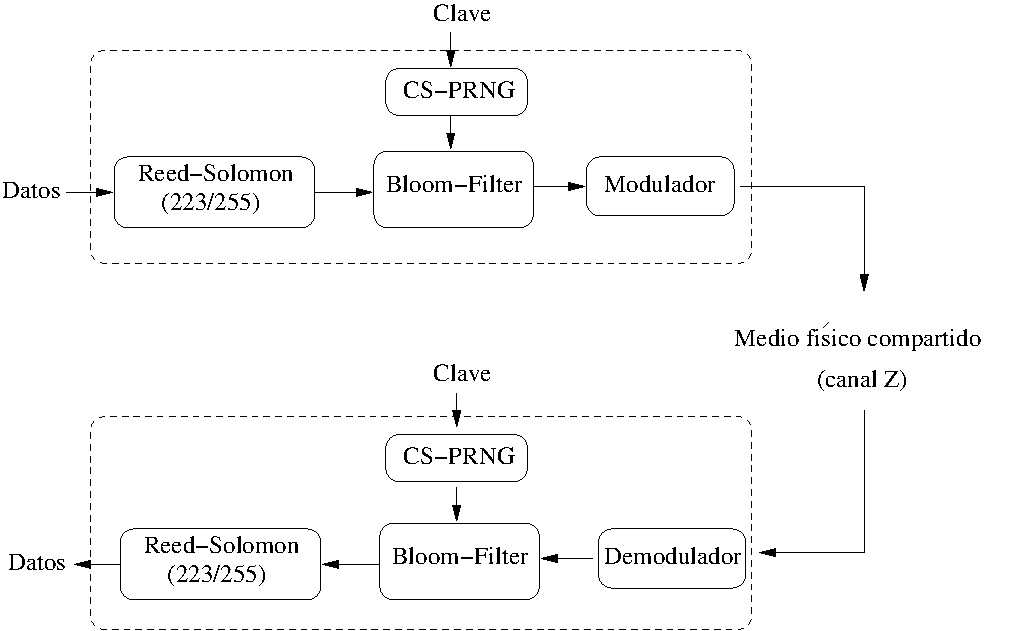
\includegraphics[width=5in]{graphs/Soft-stack3}
\caption{Diagrama esquemático del sistema de comunicaciones.}
\label{fig_comstack}
\end{figure}

\section{Códigos correctores de errores}

La selección del código corrector de errores debe ser guiada por los parámetros del sistema, teniendo en cuenta que al operar en enlaces con tasas de transmisión elevadas, una de las limitaciones más importantes es la velocidad de procesamiento de datos del sistema.

En nuestro caso, se utilizó una típica estructura de dos códigos de corrección, uno denominado código exterior (\textit{outer code}), y el segundo denominado código interior (\textit{inner code}).
La idea de utilizar dos códigos distintos es la de encadenar ambos algoritmos en serie para aprovechar las virtudes de dos tipos de corrección. Estos algoritmos se denominan códigos concatenados \cite{forney1966concatenated}. El motivo de utilizar códigos concatenados es que ciertos tipos de códigos tales como LDPC o códigos Turbo se caracterizan por poseer un piso de error elevado, que es un fenómeno donde el código pierde efectividad con relaciones señal/ruido elevadas \cite{richardson2003error}. Es para evitar esta pérdida de efectividad que se utiliza un segundo código corrector concatenado al primero, denominado código interior, que si bien no es tan efectivo con bajas relaciones de señal/ruido como el código exterior, es efectivo con señales de bajo ruido, haciendo que el sistema sea eficiente en cualquier condición.

Un parámetro importante en estos algoritmos es el retraso de codificación o latencia, es decir, la cantidad de tiempo (medida usualmente en ciclos de reloj del procesador) que demora un bit entrante a la etapa de corrección en ser procesado y salir de la misma, luego de la aplicación de la corrección de errores. Esta latencia es variable según el algoritmo. Algunos algoritmos con una latencia importante no son óptimos para utilizar en aplicaciones de bajo ancho de banda que precisan de retransmisiones o confirmaciones de los datos, ya que a cada confirmación debe sumarse también este retraso, y esto suele resultar en una disminución apreciable de la velocidad de las comunicaciones. A continuación se detalla el algoritmo de corrección seleccionado.

\subsection{Códigos de corrección Reed-Solomon}
Como código interior se seleccionó el algoritmo Reed-Solomon, un código de bloque con alta efectividad en relaciones de señal/ruido bajas. La cantidad de paridad agregada por el algoritmo, y por lo tanto, la potencia de corrección, puede ajustarse a cada aplicación, sin embargo, en computadoras digitales binarias suelen tener registros cuyo largo es múltiplo de 8 bits, por lo que es eficiente utilizar 8 bits como tamaño de símbolo en Reed-Solomon. Debido a esto, un código muy utilizado es aquel que posee un tamaño de bloque de 255 bytes y 223 bytes de datos, con 32 bytes de paridad. Estos parámetros logran que el código pueda detectar hasta 32 errores de byte y corregir hasta 16 errores dentro de los 223 bytes de datos del bloque \cite{wicker1999reed}. Al ser un estándar ampliamente utilizado, existen implementaciones eficientes de Reed-Solomon con estos parámetros específicos, tanto en software como en hardware.
Algunas desventajas de este algoritmo son:
\begin{enumerate}
 \item Elevado retraso de decodificación: Reed-Solomon es un algoritmo de complejidad temporal asimétrica. Esto significa que el retraso de codificación es mínimo (menos de 10 ciclos de reloj), pero el retraso de decodificación es elevado, pudiendo sobrepasar fácilmente los 1200 ciclos de reloj.
 \item Retraso inducido por buffer: si bien el retraso de decodificación es elevado y requiere un procesamiento no despreciable, el tiempo necesario para acumular un bloque de 256 bytes de datos en memoria para comenzar con la decodificación introduce un retraso importante, especialmente si el sistema se utiliza con bajo ancho de banda, tal como es el caso en la implementación acústica.
\end{enumerate}
 
Ambas desventajas se solucionan ajustando los parámetros de Reed-Solomon para utilizar un menor tamaño de bloque, o bien utilizando un algoritmo similar con menor tamaño de bloque, tal como BCH \cite{bose1960class}. Sin embargo, una biblioteca eficiente y disponible que permita el uso de BCH no pudo ser encontrada, por lo que la selección final fue el estándar Reed-Solomon (255, 223).

Para la simulación numérica por software se utilizó la biblioteca \textit{LibFEC} de Phil Karn~\cite{libfec}. Para la implementación en FPGA se utilizó la versión del algoritmo provista de manera gratuita en la biblioteca de núcleos de IP de Xilinx \cite{Xilinx:DS251}.

%Con posibilidad de error de simbolo P, la posibilidad de error de un codigo reed-solomon R(n/k) es:
%$$P_{rs}= \sum_{k=(\frac{n-k}{2}+1)}^{n} \binom{L}{i} * P^{i} * (1-P)^{L-i} $$
La implementación del algoritmo Reed-Solomon utilizada posee 32 bytes de paridad y 223 bytes de datos, lo que representa una adición de 14\% a la cantidad total de datos a transmitir. Este código permite corregir hasta 16 errores dentro del bloque, que pueden estar consecutivos, por lo que Reed-Solomon suele utilizarse en canales con errores de tipo \textit{``erasure''} o errores de ráfaga, donde los errores no están uniformemente distribuidos, sino que están agrupados temporal o espacialmente.

%En ciertas ona ventaja muy importante es que el codigo de correccion exterior puede facilmente detectar la presencia de un error aunque no pueda corregirlo. Esta informacion es una lista con las posiciones en las cuales se tiene la certeza que los símbolos fueron interferidos denominada lista de síndromes, y puede suministrarse al algoritmo de correccion de errores para que la capacidad de corrección del mismo puede aumentar hasta un 100\%~\cite{Moon:05}.

\subsection{Características de implementación}
Un parámetro importante en la selección del algoritmo es la facilidad de implementación sobre hardware digital. Ciertas características se vuelven importantes al pasar de implementaciones de software a hardware, tales como tamaño, memoria utilizada y velocidad máxima alcanzada con el hardware disponible, con el objetivo de que el sistema funcione a tasas de transferencia en el orden de gigabits por segundo.

A continuación, se listan las características de la implementación en hardware (FPGA) de Reed-Solomon:

El bloque de IP se denomina Reed-Solomon Encoder/Decoder 7.1 de LogiCORE IP. Con respecto al retraso, Reed-Solomon es un algoritmo de complejidad asimétrica, es decir, la complejidad espacio-temporal y ciclomática \cite{mccabe1976complexity} de los algoritmos de codificación de Reed-Solomon son diferentes a las de su correspondiente algoritmo de decodificación. En general, la decodificación es más costosa en términos de recursos de hardware y de latencia agregada al sistema. Según la especificación de esta implementación~\cite{Xilinx:DS252}, el decodificador Reed-Solomon con configuración CCSDS \cite{coding1999consultative} (que implementa el estándar (255,223)) posee un tamaño de 1364 LUTS (\textit{Look-up tables}, los elementos lógicos de la FPGA) y 3 bloques de RAM. Como comparación, el diseño completo presentado en esta tesis, posee un tamaño de aproximadamente 20000 LUTS, mientras que la FPGA utilizada posee una capacidad de 50000 LUTS. La velocidad máxima de reloj de este algoritmo en la FPGA utilizada es de aproximadamente 350 Mhz, superior a la velocidad requerida por el sistema completo a máxima velocidad, que es de aproximadamente 70 Mhz.
La cantidad de recursos utilizados por el codificador es menor: son necesarios sólo 300 LUTS y un bloque de memoria, aunque la velocidad máxima es similar~\cite{Xilinx:DS251}.

\subsection{Cálculo de latencia de la etapa de corrección de errores}
La latencia en un sistema se define como el tiempo que demora un bit en atravesarlo en su totalidad. Específicamente, el retraso en la etapa de corrección de errores representa un porcentaje importante de la latencia total en la pila de comunicación del sistema. La latencia de un algoritmo es específica a una implementación en particular.

La latencia total estará dada por el retraso introducido por la codificación sumado al retraso introducido por la decodificación, ya que los datos deben atravesar ambas etapas. Sin embargo, el tiempo de latencia en la etapa de codificación es despreciable (del orden de 5 ciclos de reloj~\cite{Xilinx:DS251}), por lo que se utilizarán sólo los valores de latencia de la etapa de decodificación. 

La latencia de la etapa de decodificación puede ser calculada de manera exacta mediante ecuaciones provistas por la hoja de datos \cite{Xilinx:DS252}. Se puede utilizar la figura \ref{fig_rslat} para obtener rápidamente el retraso de procesamiento. El parámetro $t$ se calcula como $t=(n-k)/2$ donde $n$ es la cantidad de símbolos totales en el bloque (en nuestro caso 255) y $k$ es la cantidad de símbolos de datos en el bloque (223 en nuestro caso) por lo que $t=16$.  El retraso total introducido por la decodificación estará dado por la latencia (en nuestro caso es aproximadamente 650 ciclos de reloj) sumado al retraso producto de cargar un bloque entero de datos en el decodificador. Como los datos deben ingresarse a la memoria del decodificador por medio de un bus serial de un byte de capacidad, se necesitan 255 ciclos adicionales por cada bloque. 

Sumando ambos valores, e ignorando la mínima latencia de codificación, podemos afirmar que la latencia introducida por el algoritmo Reed-Solomon en el sistema es de 900 ciclos.

\begin{figure}[t]
  \centering
  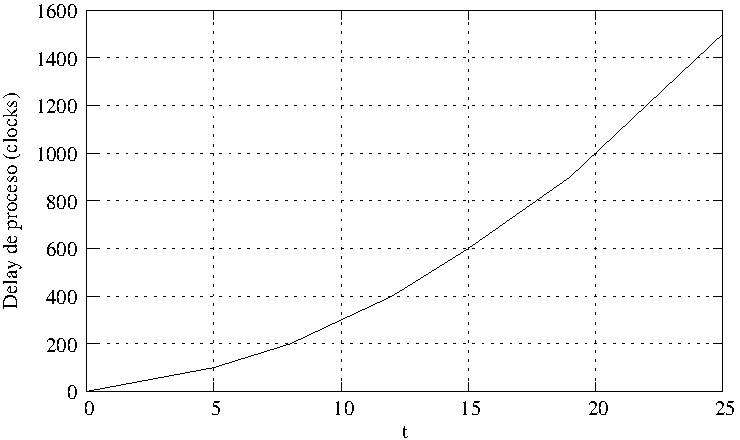
\includegraphics[width=0.8 \textwidth]{graphs/rsDelay.pdf} 
  \caption{Retraso de proceso de la implementación de Reed-Solomon utilizada~\cite{Xilinx:DS252}.}
  \label{fig_rslat}
\end{figure}


%\subsection{Optimizaciones propuestas}
% 
%Existen ciertas optimizaciones que podrían haberse realizado si se hubiera optado por implementar el algoritmo desde cero, pero que al utilizar una implementación pre-existente no se realizaron. Estas optimizaciones están relacionadas con la características del canal asimétrico, que presenta las ventajas de tener la certeza de que ciertos símbolos fueron transmitidos correctamente. Una posible optimización de Reed-Solomon para su utilización sobre canales Z se plantea para una trabajo futuro.

\section{Canal Z con filtros de Bloom}

En esta sección se describe el modelo del canal por el cual estamos transmitiendo datos, específicamente el modelo de ruido del mismo. 
Un canal de comunicaciones puede clasificarse primeramente según el tipo de información transmitida, sea binaria o analógica \cite{MacKay:2002}.
Una subclasificación del canal de comunicaciones puede realizarse según el comportamiento del ruido del mismo.

Las comunicaciones digitales suelen modelarse como un canal discreto sin memoria (\textit{discrete memoryless channel}), ya que poseen un alfabeto de símbolos de entrada $A_{x}$, que son los datos que se desea transmitir, y un alfabeto de símbolos de salida $A_{y}$ , que son los símbolos detectados por el receptor. El canal es discreto, ya que la cantidad de símbolos posible es finita. Se dice que el canal no posee memoria debido a que la probabilidad de obtener un símbolo de salida dado no depende de todos los símbolos de entrada, sino solamente del último símbolo enviado.

Otro parámetro importante que define a un canal discreto es la distribución de probabilidades condicionales $P(y|x)$ entre ambos alfabetos, es decir, la posibilidad de que al recibir el símbolo $x$ se haya transmitido el símbolo $y$. Esta distribución puede representarse como un diagrama de distribución de probabilidades (ver figura \ref{fig:canbin}) o una matriz.

De acuerdo con la distribución de probabilidades de error que mejor represente al canal físico de transmisión, el tipo de canal que mejor modela las transmisiones digitales por fibra óptica es el denominado canal Z (\textit{Z Channel}), un canal digital en el que el ruido afecta sólo uno de los símbolos binarios a transmitir.

Es este modelo de ruido nos permite innovar en el diseño de algoritmos, adaptándolos y optimizándolos para aprovechar la distribución de ruido, ya que la mayoría de los algoritmos de corrección de errores están pensados para un canal de ruido simétrico y generalmente analógico.
Empezaremos primeramente estudiando un modelo simplificado del canal por el cual vamos a trasmitir, el mencionado canal simétrico binario.

\section{Probabilidad de error del canal transmitiendo en un solo slot del frame}

\begin{figure}[t]
  \begin{center}
    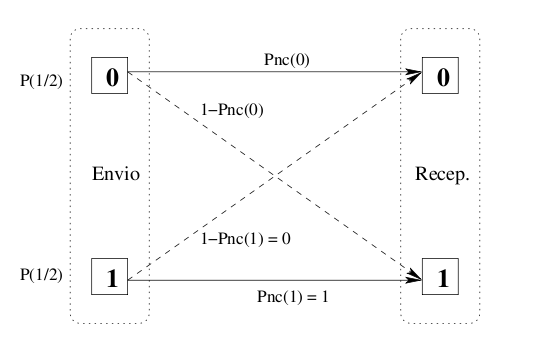
\includegraphics[scale=0.50]{graphs/canalBinario.png}
  \end{center}
\caption {Canal binario: esquema de probabilidad.}
\label{fig:canbin}
\end{figure}

Procederemos a calcular la probabilidad de no-colisión de un cliente.

Sea $M$ la cantidad de casilleros por trama y $n$ la cantidad de clientes o usuarios.

Entonces, la probabilidad de no colisión para un usuario en un slot dado es
\begin{equation}
P_{nc}=\left(\frac{M-1}{M}\right)^{n-1}
\end{equation}

Esta ecuación es válida bajo la hipótesis de que todos los clientes eligen el slot a transmitir de manera aleatoria, y de manera independiente. También consideramos que los usuarios utilizan sólo un slot.

Para simplificar, hablaremos de 'colisión' de símbolos cuando uno o más usuarios escriben en el mismo slot de un usuario y causan un error en el canal. De esta manera, en el canal Z, cuando se transmite un 1, las colisiones con símbolos transmitidos por otros usuarios no causan un error. Diremos, por tanto, que la probabilidad de no colisión de un 1 transmitido es 1, es decir, $P_{nc}(1) = 1$. Por otro lado, cuando se transmite un 0, sólo las colisiones con 1s transmitidos por otros usuarios generan error en el canal.

Siendo $P_{nc}(1)$ la probabilidad de no colisión del símbolo uno, y $P_{nc}(0)$ la probabilidad de no colisión del símbolo cero, la probabilidad total de no colisión para un usuario en un canal Z es

\begin{equation}
P_{nc}=P(1)\cdot P_{nc}(1) + P(0) \cdot P_{nc}(0) 
\end{equation}
Asumiendo que todos los usuarios transmiten un stream de datos aleatorio, tenemos que $P(1)=P(0)=\frac{1}{2}$. Entonces podemos desarrollar $P_{nc}$ como

\begin{eqnarray}
P_{nc} & = & \frac{1}{2} \cdot 1 +  \frac{1}{2} \cdot \sum_{i=0}^{n-1} 
C^{n-1}_{i} \left(\frac{M-1}{M}\right)^i  \left(\frac{1}{M}\right)^{n-1-i}  \left(\frac{1}{2}\right)^{n-1-i} 
\end{eqnarray}

La complejidad de la ecuación 3.2 se encuentra entonces en el desarrollo de $P_{nc}(0)$. Cada término de la sumatoria del segundo término del RHS de la ecuación 3.3 da la probabilidad de que $(n-i-1)$ usuarios escriban un 1 en el slot seleccionado.
El factor $C^{n-1}_{i}$ suma sobre todas las combinaciones posibles de canales que no hayan colisionado, que son hechos independientes.
\noindent Luego, $\left(\frac{M-1}{M}\right)^i$ es la probabilidad de no colisión de $i$ canales (se suma para todo posible número de canales no
colisionando: $1\leq i\leq n$, que están en otro casillero), $
\left(\frac{1}{M}\right)^{n-1-i}$ es la probabilidad de colisión de los restantes
$n-1-i$, y la colisión se produce cuando los otros canales
transmiten el símbolo $1$ cuya probabilidad es $\left(\frac{1}{2}\right)^{n-1-i}$.
%El factor combinatorio (C^{n-1}_{i}) me da la cantidad de grupos de i (o de n-1-i) usuarios de entre los (n-1) restantes puedo formar (es decir, la cantidad de formas que puedo escoger grupos de (n-1-i) personas que me sobreescriban mi querido 0).  El segundo factor me da la probabilidad de que i de los restantes (n-1) usuarios seleccionen OTROS slots. El tercer factor me da la probabilidad de que el grupo selecto de (n-1-i) usuarios elijan MI slot. Finalmente, el último factor me da la probabilidad de que los rhdp del grupo selecto de (n-1-i) usuarios escriban un 1 en MI slot



\noindent Teniendo en cuenta que $ \sum_{i=0}^{n-1}
C^{n-1}_{i} \left(\frac{M-1}{M}\right)^i  \left(\frac{1}{2M}\right)^{n-1-i}$ es la potencia $n-1$ de un binomio, reemplazando tenemos
\begin{eqnarray}
P_{nc} & = & \frac{1}{2} +  \frac{1}{2} \cdot \left(\frac{M-1}{M} + \frac{1}{2M} \right)^{n-1} \\
P_{nc} & = & \frac{1}{2} +  \frac{1}{2} \cdot \left(1- \frac{1}{2M} \right)^{n-1} \\
P_{nc} & \simeq & \frac{1}{2} +  \frac{1}{2} \cdot e^{\frac{-n}{2M}}
\end{eqnarray}

%\noindent donde la última aproximación vale para $n=M$ y $n > 2$.


Es decir, la probabilidad de no colisión depende de la relación $n/M$. Si $M>>n$, entonces $P_{nc}$ se aproxima a 1, que es una característica deseable en el sistema.
\iffalse

\vspace{5mm}

\noindent Para el caso de {\em Bloom} filters con $k$ filtros\footnote{Se envían $k$ repeticiones del bit en canales distintos, entonces basta que sólo uno de ellos sea 0 para que recibamos un 0 en un canal óptico.} la probabilidad de no colisión es:
\begin{eqnarray} 
P_{nc}^{k} & = &  P(1) \cdot P_{nc}^{k}(1) + P(0) \cdot P_{nc}^{k}(0)\\ \label{Pnc_k}
\end{eqnarray}
Sabiendo que la probabilidad de no colisión para el 0 es:
\begin{eqnarray}
P_{nc}^{k}(0) & = & 1 - \big(P_{c^k}(0)\big)^k 
\end{eqnarray}
Pero la probabilidad de colisión para el 0 cuando se transmiten $k$ copias es:
\begin{eqnarray}
P_{c^k}(0) & = & 1 - \big(P_{nc^k}(0)\big)  \enspace,
\end{eqnarray}
y que además la probabilidad de no colisión para los $k$ casilleros del Bloom
filter es
\begin{eqnarray}
P(\mbox{no col.} k) &=& P(\mbox{no col.}1)\cdot P(\mbox{no col.}2)\cdot P(\mbox{no col.}3)\cdots P(\mbox{no col.}k)\\
&=&\left(\frac{m-1}{m}\right)\cdot\left(\frac{m-2}{m-1}\right)\cdot\left(\frac{m-3}{m-2}\right)\cdots\left(\frac{m-k}{m-(k-1)}\right)\\
&=& \frac{m-k}{m} \enspace.
\end{eqnarray}
Luego la probabilidad de colisión con alguno de las $k$ copias del bit es
\begin{eqnarray}
P(\mbox{col.}k)&=& 1-P(\mbox{no col.} k)\\
&=& 1-\frac{m-k}{m}\\
&=& \frac{k}{m} \enspace.
\end{eqnarray}
Entonces reemplazamos y calculamos:
\begin{eqnarray}
P_{c^k}(0) & = & 1 - \left(\sum_{i=0}^{n-1} C^{n-1}_{i} \left(\frac{m-k}{m}\right)^i \left(\frac{k}{2m}\right)^{n-1-i} \right)  \\
& = &  1-\left( 1-\frac{k}{2m}\right)^{n-1}
\end{eqnarray}
Reemplazando esta ecuación en~\ref{Pnc_k} obtenemos:
\begin{eqnarray}
P_{nc}^k & = & \frac{1}{2} + \frac{1}{2} \left( 1- \left( 1- \left( 1- \frac{k}{2m} \right)^{n-1}  \right)^{k}  \right) 
\end{eqnarray}

Sin embargo, este calculo es incorrecto, comparandolo con los datos que da el simulador. La formula entrega valores de error menores con respecto a los reales, como se observa en la figura. 
Los trazos del mismo color corresponden a el mismo K con azul(K=1), verde (K=2) y rojo(K=4). M=256

\subsection{Entropía}

Comenzemos por lo básico:

Segun Shannon, el \textbf{contenido de informacion} h(x) de un suceso x dada la posibilidad que suceda P(x) es:
$$ h(x) = log_{2}\left(\frac{1}{P(x)}\right) $$

Y la entropia de un conjunto A, H(A) se define simplemente como el promedio del contenido de información:

$$ H(A) = \sum_{x E A_{x}} P(x)log_{2}\left(\frac{1}{P(x)}\right)$$

En un canal binario solo dos sucesos existen, uno con probabilidad p, y otro con probabilidad 1-p, por lo tanto para p siendo la probabilidad de error:

$$ H(p) = -p log_{2}(p)-(1-p)log_{2}(1-p) $$

\subsection{Entropia condicional}

Vamos a analizar la entropia de dos conjuntos X de entrada y Y de salida interrelacionados.

La entropia condicional de X dado $y=b_k$ donde $b_k$ es un valor dado, es la entropia de la distribucion de probabilidad $P(x|y=b_{k})$:
$$H(X|y=b_{k}) = \sum_{x \in A_{x}} P(x | y=b_{k})\log_2\left(\frac{1}{P(x | y=b_{k})}\right) $$

La entropia codicional de X dado Y es el promedio, sobre y, de la entropia condicional de X dado y:
$$H(X|Y) =  \sum_{xy \in A_{x}A_{y}} P(x,y)\log_2\left(\frac{1}{P(x,y)}\right) $$

\subsection{Información mútua}
La información mútua entre X e Y es:
$$I(X;Y) = H(X)-H(X|Y)$$
Mide el promedio de reduccion de la incertidumbre acerca de x que resulta de saber el valor de y, o viceversa: la cantidad promedio de informacion que x revela acerca de y.

\fi
\subsection{Capacidad de canal}

Existe una relación entre la probabilidad de error $Pb$ de un canal y la máxima velocidad de transmisión de datos posible en el mismo.
Esta relación fue estudiada por Claude Shannon en 1948 en un artículo pionero de la teoría de la información \cite{shannon48} y es conocida actualmente como teorema de Shannon-Hartley, también llamado teorema de codificación de canales con ruido (\textit{noisy channel coding theorem}).

La capacidad $C$ de un canal discreto sin memoria es la máxima información mutua entre los alfabetos $X$ de entrada e $Y$ de salida:

\begin{equation}
C = \max_{{\cal{P}}_x} I(X;Y) 
\end{equation}

Para hallar el máximo podemos derivar $I(X;Y)$ con respecto a la probabilidad $P_x$.
De \cite{MacKay:2002}, para un canal binario simétrico sin memoria con probabilidad de error $p$, la capacidad máxima $C$ es:

\begin{equation}\label{Cap}
C \approx 1 - H(p) 
\end{equation}

donde $H(p)$ es la función de entropía binaria

\begin{equation}\label{Hp}
 H(p) = [p \cdot log_2(p) + (1-p)\cdot log_2 (1-p)]
\end{equation}

Si expandimos $H(p)$ en \ref{Cap}:

$$ c = 1-\left(p \cdot \log_2\left(\frac{1}{p}\right) + (1-p) \cdot \log_2\left(\frac{1}{1-p}\right)\right) $$
Simplificada:
$$ c = 1 + p \cdot \log_2(p) + (1 - p) \cdot \log_2(1-p) $$

En la figura \ref{fig:CompBZ} puede verse la evolución de la capacidad del canal binario simétrico, que es máxima para $p=0$ y $p=1.0$, mientras que es cero para $p=0.5$, ya que con 0\% de probabilidad de error la capacidad es la máxima (no hay interferencia) y con 50\% de error la capacidad es cero y es imposible transmitir dato alguno. Quizás contra intuitivamente, con 100\% de posibilidad de error, la capacidad también es máxima, ya que equivale a invertir cada símbolo transmitido, operación que no introduce error alguno en los datos.

%Sin embargo esta capacidad es menor que la que realmente tenemos en nuestro canal, ya que un Z-channel se adecua mayormente a los medios de transmisión ópticos. Describiremos en detalle este caso especial en la siguiente sección. ??

\subsection{Canal Z}
\label{canalZ}
Un canal Z difiere de un canal binario, ya que las probabilidades de error de bit son asimétricas.
Los canales Z se usan generalmente para modelar sistemas de transmisión ópticos.

\begin{figure}[th]
  \begin{center}
    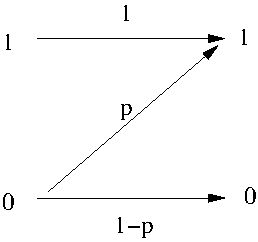
\includegraphics[scale=1]{graphs/zchannel}
  \end{center}
  \caption{Diagrama: canal Z. El diagrama superior podría representar un canal de fibra óptica donde un 1 representa el Laser encendido.}
  \label{fig:Gal}
\end{figure}

Para un canal Z, la distribución de probabilidades de la información mutua $I(X;Y)$ es diferente a la de un canal binario simétrico \cite{Tallini:02}, por lo que obtenemos un máximo diferente:

\begin{equation}\label{CapA}
C_{Z} \approx 1 - \left(\frac{1}{2}*H(p)\right)
\end{equation}

Por lo tanto, expandiendo $H(p)$ (definida en \ref{Hp}) en \ref{CapA}:

$$ C_{Z} = \log_2\left(1+(1-p) p^{p/(1-p)}\right) $$

La diferencia entre las capacidades de ambos tipos de canal puede apreciarse en la figura \ref{fig:CompBZ}. El mínimo de capacidad en el canal simétrico se da cuando $p=0.5$, mientras que en el canal asimétrico, el mínimo de capacidad se produce cuando $p=1.0$.

\begin{figure}[th]
  \begin{center}
    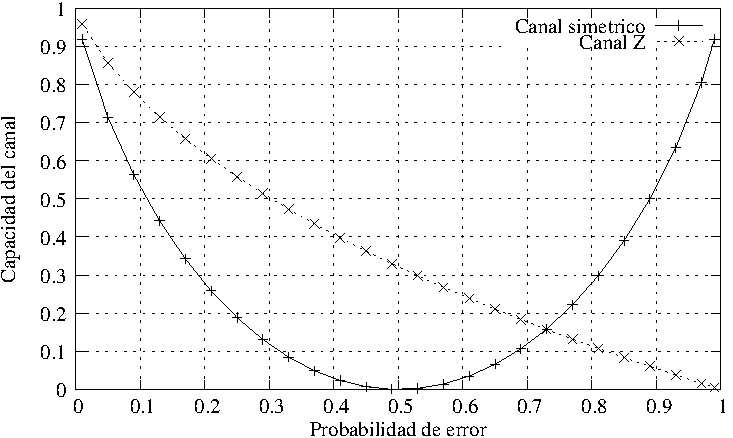
\includegraphics[scale=1.1]{graphs/grafico_comparacion_capacidad_binaria_z}
  \end{center}
  \caption{Capacidad de un canal binario simétrico con respecto a uno asimétrico o canal Z.}
  \label{fig:CompBZ}
\end{figure}


\section{Filtros de Bloom}
\label{Bloomf}
Como se discutió en la sección \ref{Seguridad} , la colisiones de símbolos son inherentes al tipo de codificación seleccionada.
En la modulación OOK (\textit{on-off keying}) utilizada en un medio óptico, sólo los ‘1’s transmitidos pueden interferir con ‘0’s. Este comportamiento puede ser modelado como un canal-Z porque la superposición de pulsos de luz individuales representando ‘1’s puede solamente ser identificados como un ‘1’s. De esto se desprende que un ‘0’ recibido es un signo inequívoco de la ausencia de pulsos en el casillero de tiempo leído.
Una buena estructura para representar este tipo de datos es el filtro de Bloom \cite{Bloom70space/timetrade-offs}, que se utiliza comúnmente como función de \textit{hash}~ \cite{song2005fast}. Dichas funciones constituyen una familia de algoritmos utilizados como tests eficientes (complejidad temporal $O(1)$) de pertenencia de un miembro en un conjunto, a diferencia de una búsqueda normal que puede tener una complejidad temporal mucho mayor (podemos citar el algoritmo de búsqueda binario, con una complejidad de $O(log_2(n))$.

La manera en que se implementó este algoritmo en el sistema propuesto se basa en copiar cada bit en $K$ casilleros de la trama transmitido, siendo la trama la representación física del filtro de Bloom.
En el extremo receptor es suficiente recibir un solo ‘0’ entre las $K$ copias del bit, para inferir que el bit original era originalmente un ‘0’, mientras que si el bit original era un ‘1’, las colisiones no tienen efecto debido a la naturaleza del canal-Z.

En la figura \ref{fig:Bloomf} puede apreciarse gráficamente como se utiliza un filtro de Bloom para la transmisión de 12 clientes con una repetición $K=3$. 

\begin{figure}[th]
  \begin{center}
    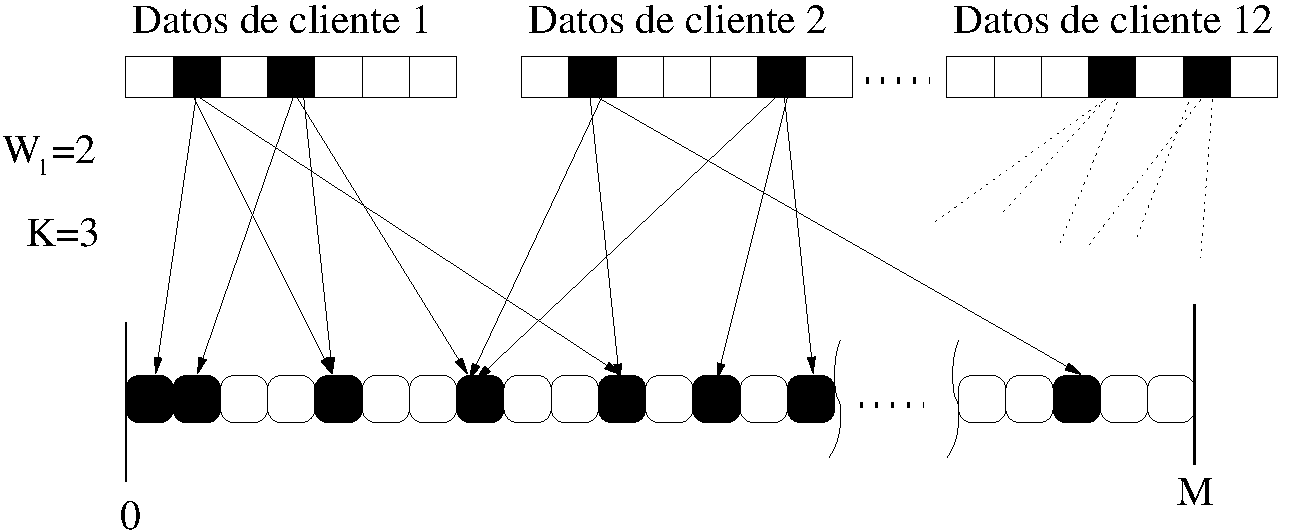
\includegraphics[scale=0.55]{graphs/frame-sp}
  \end{center}
  \caption{Filtro de Bloom. M es el largo de la trama. $W_1$ es el peso de Hamming mínimo. El parámetro K es el número de repeticiones.}
  \label{fig:Bloomf}
\end{figure}

%As discussed in section 2, this leads to collisions. Since the modulation format is OOK, only transmitted ‘1’s can interfere with ‘0’s.
%This behaviour can be modelled as a Z-channel because the superposition of individual light pulses representing ‘1’s
%can only be identified as a ‘1’, but a received ‘0’ is an unmistakable sign of the absence of pulses in a given time casillero.
%We found that the Bloom filter [2] provides a convenient structure to correct for errors in this type of channel. This
%technique is borrowed from hashing algorithms and is used to test whether an element is member of a given set. The
%way that we implement this algorithm relies on copying every bit in K casilleros of the transmitted frame. On the receiving
%end it is sufficient to receive a single ‘0’ out of K copies in order to correctly retrieve the original transmitted ‘0’,
%whereas collisions have no effect on ‘1’s.

\subsection{Filtros de Bloom encriptados}

En esta etapa se realiza la encriptación de los datos, reemplazando el algoritmo de hashing que selecciona las posiciones de los datos dentro del filtro de Bloom por una función pseudoaleatoria criptográficamente segura, de modo que los bits de datos de los diferentes clientes se posicionan aleatoriamente en la trama, y sólo es posible decodificar los datos si se tiene exactamente la misma secuencia pseudoaleatoria con que fueron posicionados originalmente. Como esta secuencia está determinada por la semilla del algoritmo PRNG, los participantes deberán compartir esta semilla previamente, que es el equivalente a una clave o password simétrico. 

Desde el punto de vista de la modulación, el algoritmo PRNG selecciona la posición temporal dentro de la trama, por lo que este esquema es equivalente a una transmisión time hopping, con la única salvedad de que el algoritmo de filtro de Bloom requiere $K$ repeticiones de los datos para poder recuperarlos de colisiones en la recepción.

Para poder decodificar los datos en el filtro de Bloom receptor es necesario que todos los participantes posean la misma secuencia pseudoaleatoria, es decir, la misma clave o semilla generadora \ref{PRNGs} del mismo PRNG utilizado para codificar los datos, y todos deben estar sincronizados a nivel de trama con el nodo originante. Las tramas del cliente originante y el receptor deben empezar y terminar al mismo tiempo para poder regenerar exactamente todas las posiciones en donde se transmitieron los datos. 

Sin embargo, los demás clientes que utilizan el medio compartido sólo causan interferencia y por lo tanto la sincronización a nivel de trama sólo es necesaria entre los clientes que deseen compartir el canal encriptado. Esto reduce los requerimientos de sincronización y simplifica la implementación de la red.

Finalmente, es deseable, pero no necesario, que todos los clientes mantengan una sincronización a nivel de bit, es decir, que los tiempos de transmisión de todos los clientes estén suficientemente alineados para que el casillero de un cliente sólo pueda superponerse con otro casillero de otro cliente y le cause un solo error de bit. Si esta sincronización no se mantiene, un casillero podría interferir con dos casilleros de otro cliente que está desalineado con respecto al primero, provocando dos errores en lugar de uno solo y aumentando los requerimientos de corrección de errores en el sistema.

\section{Minimización de peso de Hamming}
%% extraido de dline-pub.text
\label{miniham}
El esquema propuesto, basado en time-hopping CDMA, utiliza la interferencia entre símbolos para obtener confidencialidad, ya que los datos de los otros usuarios actúan efectivamente como ruido.
La interferencia intersímbolo, como fue discutida en la sección \ref{cap2:ECC}, causa errores en la comunicación que deben ser corregidos. Para reducir la interferencia, no es aconsejable modificar o introducir patrones en el generador criptográficamente seguro de números aleatorios, ya que comprometería la seguridad de todo el sistema al existir la posibilidad de introducir factores que permitan predecir las posiciones de los símbolos (ej. usando códigos ortogonales como en Ref.~\cite{Nadarajah2006}.), efectivamente dejando de ser criptográficamente seguro.

%This channel presents a Shannon limit of $ C_{Z} = \log_2\left(1+(1-p) p^{p/(1-p)}\right),$ where $p$ is the probability of error~\cite{Tallini:02}.

Considerando que el medio de transmisión se adecua a un canal Z, se propone aprovechar la naturaleza asimétrica de este tipo de medio, en donde solamente el símbolo ``1'' causa interferencia. \footnote{Aunque en un sistema de comunicaciones ópticas real, existe una pequeña diferencia ya que el nivel de ``0'' no es representado con una potencia de cero Watts.}
En otras palabras, la interferencia de un canal Z es proporcional al peso de Hamming ($HW$) del símbolo transmitido.
En esta sección se presenta un algoritmo que minimiza este valor, con el objetivo de causar menor interferencia. El algoritmo de minimización de peso de Hamming consiste en una codificación en donde cada símbolo binario es convertido en un equivalente de mayor longitud, que posee una mínima cantidad de dígitos en ``1''. Aplicando esta codificación y transmitiendo el símbolo resultante, se obtiene una menor interferencia, siempre y cuando el medio de transmisión pueda modelarse como un canal Z.
Intuitivamente, expandir el símbolo original a uno de mayor longitud reduciría el ancho de banda del canal; pero como las simulaciones numéricas muestran (ver sección \ref{simulations}) a medida que la interferencia intersímbolo disminuye, el ancho de banda adicional utilizado por los algoritmos de FEC también se reduce, compensando por el incremento del largo del símbolo, y logrando un mayor ancho de banda efectivo del sistema.
Podemos decir que un número binario normal de largo $L$ posee un $HW$ variable, con $L/2$ siendo el promedio, cero siendo el mínimo y $L$ siendo el $HW$ máximo.
La técnica de reducción logra que $HW=2$, siendo este valor un balance apropiado entre la reducción de interferencia y el largo de símbolo.
Adicionalmente, es deseable en un sistema de seguridad que no se revele ninguna información acerca de los símbolos transmitidos. Por ejemplo, si transmitiéramos el número cero, representado por todos sus dígitos en cero, sería trivial identificarlo debido a la ausencia de dígitos en uno, condición fácilmente detectable. Para evitar este tipo de actividad maliciosa o ``ataques'' que utilizan análisis estadísticos de los datos, la codificación exige que el peso de Hamming sea fijo en todos los símbolos. Esto causa una ligera pérdida en el ancho de banda, pero hace imposible inferir cualquier tipo de información acerca de los datos transmitidos analizando estadísticas de tráfico.

\begin{table}[t]
\begin{center}
\begin{tabular}{c c c}
Datos & entrada HW= 0 a 3 & Expandida HW=2\\
\hline\hline
0 & 000 & 00011\\
1 & 001 & 00110\\
2 & 010 & 00101\\
3 & 011 & 01100\\
4 & 100 & 01010\\
5 & 101 & 01001\\
6 & 110 & 10001\\
7 & 111 & 10010\\
\end{tabular}
\caption{Tabla de minimización de Hamming para símbolos de 3 bits. Esta tabla puede utilizarse para convertir datos de entrada (números del 0 al 7 y su representación binaria) en su representación con peso de Hamming minimizado, en la tercer columna. El peso de Hamming de los símbolos de entrada es variable de 0 a 3, y el de salida es siempre 2.}
\label{hwtable}
\end{center}
 \end{table}
 
\section{Expansión de símbolo}
La minimización del peso de Hamming conlleva una necesaria conversión del símbolo original a otro que tendrá mayor longitud, es decir, una expansión del símbolo.
Esta operación puede realizarse de muchas maneras, pero un algoritmo eficiente es la tabla de lookup (ver tabla~\ref{hwtable}), donde un símbolo de largo L es utilizado como el índice en una tabla, y la salida se encuentra en la segunda columna de la misma tabla, donde estará almacenado el símbolo expandido de largo N, siendo que $N\textgreater L$.
Por motivos prácticos y de optimización, es deseable que $L$ sea múltiplo de 8. Al aplicar la minimización de $HW$ a símbolos de 8 o 16 bits de longitud, son necesarios 256 o 65536 símbolos de salida, respectivamente, cada uno con un $HW=2$. En el caso de símbolos de entrada de 8 bits, la longitud del símbolo de salida será de 363 bits, mientras que, para 8 bits de entrada, el símbolo expandido con $HW=2$ tendrá 24 bits de longitud.
Puede observarse que el número de símbolos únicos con $HW=2$ y $N=363$ no es exactamente 65536 sino 65703. Esto significa que la tabla de expansión no es única, sino que existen muchas tablas funcionalmente equivalentes que pueden seleccionarse. Cada tabla posible producirá un conjunto único de símbolos con $HW=2$, por lo que a pesar de ser equivalentes, los nodos participantes deberán necesariamente utilizar idénticas tablas para la codificación y decodificación.
%In general more bits transmitted per frame the more efficient the protocol will be. \textbf{PORQUE IN GENERAL? CUANDO FALL
\begin{figure}[!t]
  \centering
    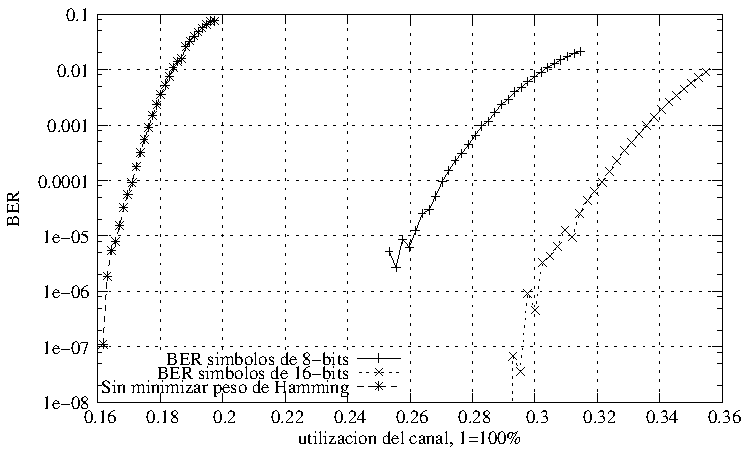
\includegraphics[width=6in]{graphs/BERvsChannelES2}
    \caption{Performance del sistema con respecto a la expansión de símbolo. Simulación numérica de un enlace de 10 Gbps con 128 clientes, M=4096 y K=9.}
    \label{BERvsExpansion}
\end{figure}

La Figura \ref{BERvsExpansion} muestra tres simulaciones: una sin expansión, otra con una expansión de 8 bits y otra de 16 bits. En dicha figura se muestra el BER en función de la utilización del canal (el porcentaje real de uso por la totalidad de los clientes cuando se elimina todos los bits extras de las codificaciones, es decir, la capacidad que la suma de usuarios vería sin este sistema). Como se puede apreciar, hay una mejora substancial en el aprovechamiento del canal: para un BER de $10^{-6}$ tenemos 0.16, 0.25 y 0.3 aproximadamente. Es decir que con 8 bit mejoramos un $50\%$ del original, y con 16 bis un $87\%$.


\section{Probabilidad de colisión de filtro de Bloom con expansión de símbolo}

%newJIS_140512
En esta sección, presentaremos una estimación analítica de la probabilidad de error de bit, tomando en cuenta sólo las interferencias de otros usuarios en la red.
No consideraremos ninguna corrección de etapas o algoritmos adicionales como Reed-Solomon, o interferencias producidas en el medio físico.
Como se explicó en la sección \ref{Bloomf}, cada usuario agrupa sus bits de información en paquetes o tramas de largo $n$. Cada paquete es codificado utilizando exactamente $m_{1}$ unos y $m_{0}$ ceros, siendo $m$ la cantidad de bits de la trama, donde $$m=m_{1}+m_{0}$$.

Debido a la utilización del filtro de Bloom, cada uno de los $m$ dígitos binarios resultantes es repetido $K$ veces en posiciones elegidas aleatoriamente en la trama de largo $M$. Las K repeticiones de un dígito binario pueden colisionar con otras repeticiones del mismo dígito, con repeticiones de otro dígito o bien con dígitos pertenecientes a otro cliente.
Llamaremos $N$ al número de usuarios activos. Para estimar la tasa de error o BER (Bit Error Rate) del sistema y simplificar los cálculos, asumiremos lo siguiente:

\begin{enumerate}
 \item Las tramas de diferentes usuarios están sincronizadas, es decir, cada usuario participante del canal de comunicaciones recibe la misma trama en el mismo orden, y cada trama contiene (incluyendo colisiones) $W_0 = N\cdot K\cdot m_0$ ceros y $W_1 = N\cdot K\cdot m_1$ unos.
 \item No incluiremos en el análisis la posibilidad de corrección de errores debido a que, en general, 
 \begin{equation}
\nchoosek{m}{m_1} > 2^n.
\end{equation}
Específicamente, cada vez que una secuencia errónea de $m$ dígitos binarios es recibida con más de $m_1$ unos, se decodifica como una cadena de bits aleatoria de largo $n$.
Por lo tanto, el número esperado de errores será $n/2$.
\end{enumerate}

Definiremos las siguientes probabilidades: 
$P_{s1}$ como la probabilidad de sobre-escribir con unos las $K$ repeticiones de por lo menos uno de los $m_0$ ceros.
$P_{st}$ como la probabilidad de sobrescribir con unos todas las $K$ repeticiones de uno de los $m_0$ ceros.

Entonces, el BER está dado por
\begin{equation}
%\text{BER} = \frac{n}{2}\prob{\text{sobre-escribir con unos las $K$ repeticiones de por lo menos uno de los $m_0$ ceros}}.
\text{BER} = \frac{n}{2}P_{s1}.
\label{eq:ber_01}
\end{equation}
Por la cota de la unión (union bound), 
%\begin{multline}
\begin{equation}
%\prob{\text{sobrescribir con unos las $K$ repeticiones de por lo menos uno de los $m_0$ ceros}}\leq \\
%\leq m_0\prob{\text{sobrescribir con unos las $K$ repeticiones de uno de los $m_0$ ceros}}.
P_{s1}\leq P_{st}.
\label{eq:union_bound}
\end{equation}
%\end{multline}
Por lo tanto, prestemos atención a uno de los $m_0$ ceros. Si los $W_{1}$ transmitidos (por todos los usuarios) ocupan $s$ casilleros y las $K$ repeticiones del cero dado usa $r ( \leq K)$ casilleros, entonces una condición necesaria para el error es que $s \geq r$. Entonces, asumimos que existan $s$ unos en una trama de $M$ bits. Dados $r$ lugares en la trama, la probabilidad de que los unos ocupen esas $r$ posiciones está dada por 
\begin{equation}
z_{r,s} = \frac{\nchoosek{M-r}{s-r}}{\nchoosek{M}{s}}= \frac{\frac{(M-r)!}{(M-s)! (s-r)!}}{\frac{M!}{(M-s)!s!}} = \frac{(M-r)!}{M!}\frac{s!}{(s-r)!}\approx (\frac{s}{M})^r,
\end{equation}

Suponiendo que $N,s\gg r$, si $M \gg K$, no es difícil ver que las $K$ repeticiones de un cero dado ocupan $\mu_{R} \approx K$ casilleros en promedio. También puede demostrarse que el número promedio de casilleros ocupados por los $W_{1}$ unos transmitidos por todos los usuarios es

\begin{equation}
\mu_{S} \approx M (1-e^{-W_1/M})
\end{equation}
 
De esas ecuaciones, una estimación de la cota superior del BER para un determinado usuario es
\begin{equation}
\text{BER} \approx \frac{n}{2} m_0 z_{\bar{R},\bar{S}} \approx \frac{n}{2} m_0 \left(1-e^{-W_1/M}\right)^K.
\end{equation}

La figura \ref{BERvsK} muestra la estimación en función de $K$ para $M=2014$, $m_{0} = 22$, $m_{1} = 2$, $n = 8$ y $N=38$. Es interesante notar que existe un valor óptimo de la tasa de repetición $K$ que minimiza la tasa de error. Este resultado es relevante en el diseño de un sistema de comunicaciones. Debido a los bajos valores de BER alcanzados, es posible utilizar en la siguiente etapa algoritmos eficientes que aceptan bajos límites de error, tal como Reed-Solomon, para reducir aún mas el BER total de sistema y asi llevarlo a tasas aceptables para aplicaciones prácticas.

\begin{figure}[!t]
  \centering
    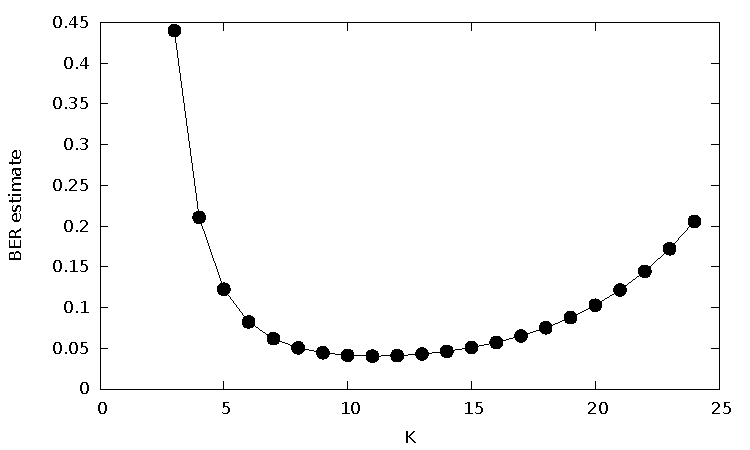
\includegraphics[width=5in]{graphs/Kcalc}
    \caption{Estimación de BER vs. tasa de repetición de filtro de Bloom K.}
    \label{BERvsK}
\end{figure}

\section{Códigos de pseudoruido}
Como se explica en la sección \ref{PRNGs} la seguridad del sistema depende de la correcta selección e implementación de un algoritmo de PRNG criptográficamente seguro \textit{(CS-PRNG)}.
El sistema impone una restricción adicional a esta etapa, ya que además de cumplir con todas las propiedades de un CS-PRNG, se debe seleccionar un algoritmo eficiente ya que se necesitará generar una posición aleatoria por cada bit que se desea transmitir. Por lo tanto, es deseable maximizar la cantidad de bits por ciclo de reloj que el CS-PRNG es capaz de generar.
En el caso de la implementación para el transceptor óptico sobre una FPGA, el algoritmo seleccionado para el prototipo inicial fue el denominado ARC4, debido a la simplicidad, bajo consumo de recursos de hardware y alta velocidad del mismo  \cite{Menezes:1996:HAC:548089}. Si bien existen implementaciones de alta performance \cite{10.1109/TC.2012.19}, estas no son fácilmente accesibles ni disponibles, por lo que se reimplementó este algoritmo íntegramente, utilizando el lenguaje de descripción de hardware Verilog \cite{thomas2002verilog}, utilizando optimizaciones para lograr la performance deseada de 1 byte pseudoaleatorio generado por cada ciclo de reloj. Es necesario tener en cuenta es que ARC4 es un algoritmo relativamente anticuado y recientemente varios ataques estadísticos han puesto en duda su utilización como generador criptográficamente seguro \cite{Sepehrdad:2011:SAR:2008684.2008712}, por lo que en implementaciones futuras es recomendable que sea reemplazado por un algoritmo criptográfico moderno.

En las implementaciones de software o acústicas, el poder de procesamiento necesario para esta etapa se reduce, ya que la velocidad de reloj de un CPU suele ser elevada con respecto a la velocidad posible en este medio de trasmisión, por lo que no es necesario que el algoritmo PRNG tenga un rendimiento elevado.


\subsection{Aplicación al algoritmo de filtro de Bloom encriptado}

Este algoritmo asigna los tiempos de transmisión de $r$ clientes, seleccionándolos entre $M$ posiciones, correspondientes a los $M$ casilleros dentro de la trama de transmisión.
La cantidad posible de combinaciones de $M$ posiciones entre todos los clientes es de $ _{M}P_{r} = \frac{M!}{(n-r)!} $.
Consideraremos que un ataque a este algoritmo fue exitoso cuando un atacante puede inferir la serie de posiciones $M$ para un cliente, obteniendo así todos sus datos.

Existe un algoritmo de selección de $M$ que suponemos no posee ninguna debilidad, es decir, selecciona $r$ conjuntos de $M$ posiciones tal que, aún si el atacante pudo adquirir un número arbitrario de las posiciónes de transmisión pasadas, no puede predecir ninguna de las posiciones futuras.

Esto puede cumplirse simplemente asignando a cada canal de transmisión seguro su propio algoritmo generador pseudoaleatorio criptográficamente seguro, o bien el mismo algoritmo utilizando claves diferentes. Esto provocará colisiones entre los clientes, es decir, al asignarse posiciones de transmisión de manera aleatoria, existirán coincidencias donde a dos o más clientes se les asignará el mismo casillero dentro de la trama. Esto es resuelto mediante corrección de errores en capas superiores y para el cálculo del parámetro de seguridad se despreciará este efecto.

Dadas las siguientes suposiciones:
\begin{itemize}
 \item El algoritmo de selección pseudoaleatorio no tiene debilidades.
 \item El atacante no posee control de los datos a transmitir, y estos son totalmente aleatorios.
\end{itemize}

Un atacante podria tratar de predecir el conjunto de posiciones $n$ de un cliente, para obtener sus datos. Para ello, deberá probar exhaustivamente todo el conjunto de $ _{M}P_{r}$ sobre una trama capturada, o bien probar todas las combinaciones posibles de la clave del generador pseudoaleatorio. De esto se desprende que si $largo(clave)>128\ bits$ y $M>128$ se considera que el algoritmo cuenta con un nivel de seguridad denominada ``fuerte'', ya que una complejidad temporal de $2^{128}$ es considerada segura al momento de la escritura de esta Tesis \cite{eastlake2005s}.

\subsection{Problemas de símbolos con peso de Hamming variable}
En la sección anterior se nombraron dos condiciones necesarias. La primera condición, la carencia de vulnerabilidades en el algoritmo CS-PRNG, es necesaria e inevitable por motivos obvios. Sin embargo, es posible eliminar la segunda condición, de precisar datos totalmente aleatorios, realizando una modificación a la tabla de expansión. Esto es posible ya que la segunda condición es sólo necesaria para prevenir el siguiente escenario donde la seguridad falla:

Supongamos que se desea transmitir dos bytes:
\begin{itemize}
 \item El byte 0 ($00000000$ en representación binaria) 
 \item Y el byte 255 ($11111111$ en representación binaria)
 \end{itemize}

La tabla de expansión convierte los símbolos de 8 bits en símbolos de 16 bits, con peso de Hamming $HW<=2$.
Supongamos que la tabla asignó al valor 0, el símbolo $0000000000000000$ y al valor 255 el símbolo $0000100010000000$. Ambos símbolos de salida cumplen con la condición de $HW<=2$. Al transmitirse estos bytes, las posiciones son aleatorizadas y transmitidas.

Ignorando momentáneamente las colisiones, un atacante que observa el tráfico puede reconocer qué byte esta siendo transmitido, aún cuando la posición de cada bit este aleatorizada, simplemente contando la cantidad de unos, es decir, el peso de Hamming variable está revelando al atacante información acerca de los datos transmitidos, aún cuando los símbolos fueron permutados.

Éste ataque puede eliminarse generando una tabla de expansión cuyo peso de Hamming de símbolos de salida sea estrictamente un valor fijo. Es decir, para evitar el ataque en el ejemplo anterior, los símbolos de salida en lugar de tener $HW<=2$ deben cumplir con la condición de $HW=2$. 

De esta manera, al convertir los datos de entrada en símbolos uniformes con el mismo largo y el mismo peso de Hamming \footnote{Si el peso de Hamming es $P$, el atacante podrá observar un peso de Hamming de $1$ hasta $P$, y no siempre $P$, esto es debido a las colisiones de bit que un símbolo transmitido por un cliente tendrá con sí mismo.}, los bits de salida del algoritmo serán completamente aleatorios sin importar los datos de entrada y el atacante no podrá inferir ninguna información acerca de la comunicación.

\section{Resumen del sistema completo}
%% De orte.tex
El sistema propuesto, cuyo diagrama de alto nivel se muestra en la figura \ref{fig_comstack}, está compuesto primeramente de una capa de acceso, donde se encuentra la implementación de la codificación CDMA y la corrección de errores, y una capa física basada, o bien en una red óptica con similitudes a redes PON \ref{defPON} , o una red acústica de tipo difusión (\textit{broadcast}).
La capa de acceso está implementada utilizando técnicas CDMA del tipo time-hopping, donde cada uno de los clientes posibles codifica su información en bits y los transmite en un casillero seleccionado de manera aleatoria dentro de una trama de $M$ casilleros\footnote{ El parámetro $M$ debe optimizarse en función del nivel de error aceptable y la máxima cantidad de clientes soportados.}. De esta manera, ocurrirán múltiples colisiones entre diferentes ONUs \textit{(optical network unit)}, pero los errores causados por estas colisiones serán corregidos por la capa de corrección que garantiza una transmisión de datos confiable. Aunque es imposible eliminar totalmente los errores, consideramos una transmisión con un BER de 10e-12 como libre de errores.

Si bien existe el requerimiento de que todos los clientes comunicantes deben estar sincronizados a nivel de trama para regenerar correctamente las posiciones de transmisión, esta sincronización no es necesaria para clientes que no participen del canal encriptado.
Un cliente $X$ puede recibir mensajes de otro cliente $Y$ si y sólo si $X$ posee la {\em clave} de $Y$, y viceversa. De esta manera, si un cierto grupo de clientes desea comunicarse sobre un canal encriptado, es necesario cada cliente en el grupo conozca la {\em clave}. El canal encriptado que se forma entre los clientes forma un ``dominio de difusión'' ya que todos los datos que transmita un cliente serán recibidos sólo por los otros clientes participantes del dominio. Este dominio es análogo al sistema VLAN \textit{(Virtual Local Area Network)} de particiones lógicas de red.

Los datos de los clientes se codifican con las siguientes técnicas de corrección de errores: Reed-Solomon ($223/255$) (ver \cite{Moon:05} y sus referencias), y un filtro de Bloom\cite{Bloom70space/timetrade-offs}. 

En principio, se utilizó un algoritmo LDPC \ref{defLDPC} (Con matriz de $1024\times512$) pero fue descartado en posteriores iteraciones del diseño, ya que al agregar la optimización de la expansión de símbolo al filtro de Bloom, se incrementó la capacidad de corrección del mismo y pudo eliminarse la etapa de corrección de errores de tipo LDPC, con el consiguiente aumento de la capacidad total del sistema.

En la selección de los algoritmos de corrección de errores siempre se utilizó el canal Z como modelo del canal de comunicaciones. %que posee un limite de Shannon de $ C_{Z} = \log_2\left(1+(1-p) p^{p/(1-p)}\right),$ donde $p$ es la posibilidad de recibir un error al transmitir un bit. Este limite de capacidad es menor que el límite en una canal simétrico sin memoria \cite{Tallini:02}.

\section{Aplicación en distintos medios físicos}
Al poseer una fuerte capacidad de corrección de errores, la arquitectura del sistema lo hace confiable frente a todo tipo de interferencias de la capa física, por lo que modificando la etapa de modulación pueden utilizarse diferentes medios físicos, siempre que los mismos puedan modelarse como un canal Z.
\begin{figure}[t]
  \centering
      \subfloat[Distribución via acoplador tipo estrella 1]{{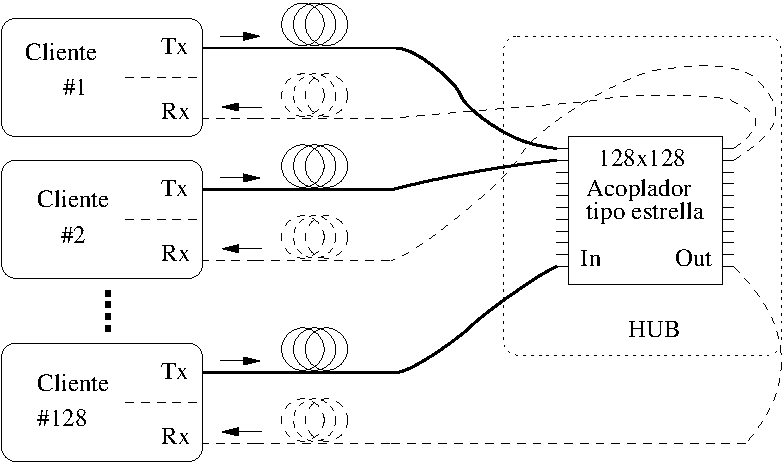
\includegraphics[width=0.62 \textwidth]{graphs/StarCoupler} }}%
    \qquad
    \subfloat[Distribución via EDFA]{{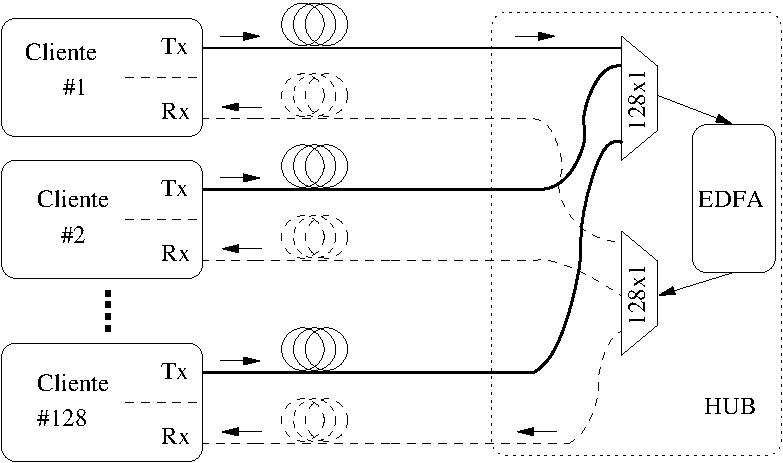
\includegraphics[width=0.62 \textwidth]{graphs/EDFA} }}%
    \caption{Diseño de red propuesto para la capa óptica: un acoplador de tipo estrella es la base para la arquitectura de red en distancias inferiores a $10~\mathrm{km}$. Para extender el alcance de la red, un amplificador óptico del tipo EDFA \textit{(Erbium-Doped Fiber Amplifier)} puede ser utilizado en el concentrador central.}
    \label{arch:fig1}
\end{figure}

\subsection{Redes ópticas}
% de orte.text



%\begin{figure}[t]
%  \centering
%  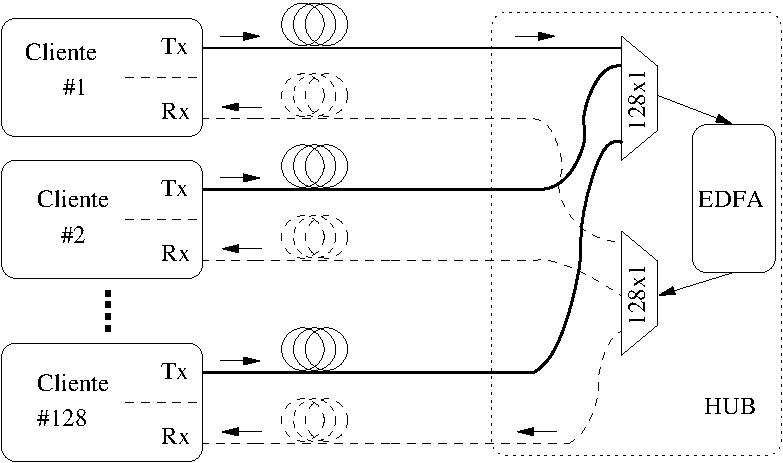
\includegraphics[width=0.48 \textwidth]{graphs/EDFA}
%  \caption{Para distancias superiores a $10~\mathrm{km}$ la red requiere amplificación provista por un EDFA.}
%  \label{arch:hub_edfa}
%\end{figure}


%\begin{figure}[!t]
%  \centering
%    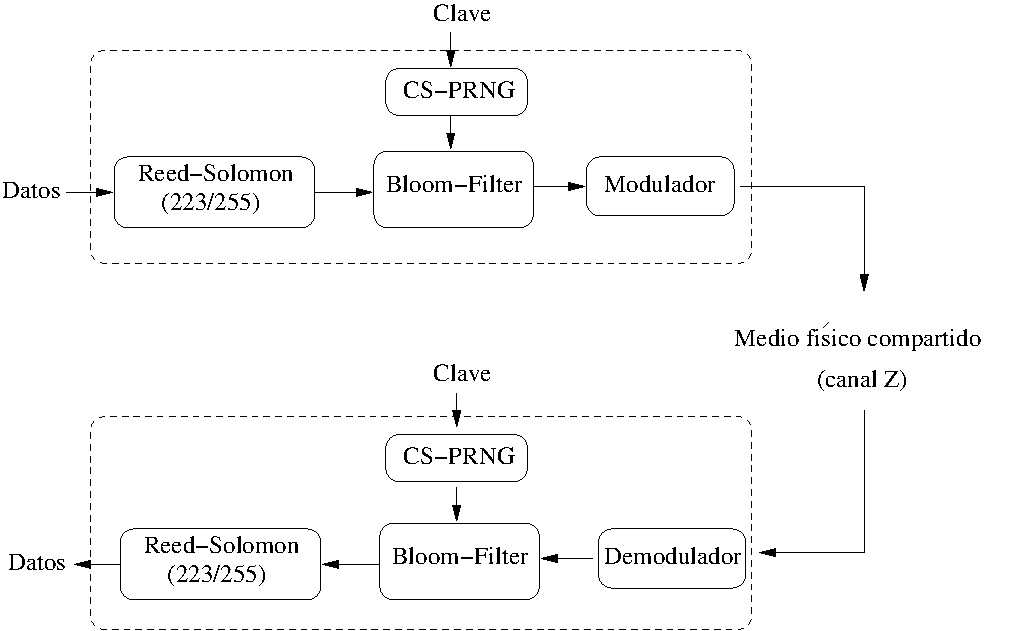
\includegraphics[width=5in]{graphs/Soft-stack3}
%    \caption{Diseño de red propuesto: Pila de comunicaciones}
%    \label{arch:chain}
%\end{figure}
% Fiber		Es grave el efecto de la dispersion?  Sugerimos dispersion shifted G.653? O son muy caras?
% splitter	No 1x128 commercially available (attenuation $\leq 27\,dB$)
% DFB		http://cess-dk.com/gfx/upload/PX2-1541SF.pdf ( min $\simeq-1\,dB$)
% APD		http://pdf.dzsc.net.cn/200810212/286762.pdf ( max $\simeq-27\,dB$)
% EDFA		http://www.lambdaphoto.co.uk/pdfs/EDFADatasheet.pdf

Al adaptar el sistema propuesto a una red óptica, la topología física debe ser de tipo estrella (ver figura \ref{arch:fig1}) donde splitters ópticos redistribuyen el tráfico proveniente de cada ONU a todo el resto de los terminales, permitiendo comunicaciones punto a punto así como punto a multipunto, con una cantidad máxima de hasta $128$ ONUs simultáneas. Este límite esta dado por las atenuaciones causadas por la fibra óptica y por el concentrador que el sistema debe ser capaz de compensar mediante amplificación.

%Traffic redistribution is made by optical splitters at the redistribution hub that introduces high attenuation to optical streams.
Un amplificador óptico de tipo EDFA \textit{(Erbium-Doped Fiber Amplifier)} localizado entre los splitters incrementa la potencia óptica para compensar las perdidas en la red, aunque esto es solamente necesario en distancias entre clientes superiores a 10 km.

La modulación utilizada para las señales ópticas es RZ o \textit{Return to Zero}, con velocidades previstas de hasta $10$~Gbps, utilizando un Láser DBF \textit{(Distributed Feedback)} de $2$~dBm de potencia y $1550$~nm de color/frecuencia. Estos parámetros permiten una transmisión de hasta $10$~km entre los nodos si se utiliza fibra óptica mono modo estándar (ITU-T G.652).

En el concentrador, un splitter de $128\times 1$ concentra el tráfico de todos los ONUs y es luego redistribuido por el correspondiente splitter de $1\times 128$, canalizando el tráfico combinado de cada ONU a través de las fibras ópticas. Este splitter permite tener hasta 128 ONUs en el sistema.

La atenuación de los splitters centrales ($\simeq25$~dB cada uno) sumada a la atenuación propia de la fibra óptica ($\simeq2$~dB por tramo) y pérdidas por inserción (aproximadamente $\simeq1$~dB) contribuyen a la elevada atenuación que el amplificador debe compensar ($\simeq28$~dB).

De utilizarse sin ningún tipo de amplificación, la atenuación que una señal sufriría entre dos ONUs es la suma de la atenuación de ambos tramos, es decir $\simeq56$~dB, que es un valor que supera el límite de la tecnología de detección comercial disponible al momento de la escritura de esta Tesis, teniendo en cuenta potencias de transmisión máximas de 2 dBm.

Sin embargo, es posible utilizar etapas de amplificación intermedias para obtener niveles de señal adecuados. Para proveer la amplificación requerida, un EDFA con $\geq27$~dB de ganancia es colocado entre ambos splitters. Este EDFA incrementa la potencia del tráfico a la salida del primer splitter, elevando la potencia de cada '1' de $\simeq-26$~dBm a $1$~dBm a la entrada del segundo splitter, que será atenuada nuevamente a un nivel de potencia de $-27$~dBm, valor dentro de los parámetros aceptables de un fotodetector de alta sensibilidad (aproximadamente $-28$~dBm~\cite{comapd}).

%La potencia máxima de salida del PD no es un parámetro crítico ya que simulaciones [CUALES?] muestran que solamente se producirán colisiones de hasta diez `1' en un casillero, y esto con una posibilidad extremadamente baja. -- eliminado por carencia de simulaciones

Aún considerando una ganancia de EDFA constante, la potencia óptica a la entrada del detector PD sería menor ($-17$~dBm) que la requerida por dispositivos comerciales ($\sim -5$~dBm).
El nivel de bit `0' es dado por la adición de todos los bits `0' transmitidos por las $128$~ONUs. Por lo tanto, el nivel de decisión del receptor debería ser capaz de separar entre este estado (la suma de los bits `0') y aquel de un simple ONU transmitiendo un solo bit en `1'.
De esto se desprende que la potencia de transmisión del bit `0' debe ser la menor posible, o lo que es lo mismo, la \textit{relación de extinción} del láser DBF debe ser alta.
%El radio de extinción (`1'$/$`0' radio de potencia pico) mínimo requerido por el sistema se discute en las simulaciones numéricas a continuación:

% As collisions occur in this scheme minimal powers are such for the case of a single active Tx in a bit casillero. In a bit casillero with collisions (two or more `1' bits) power increase could be a concern to APD operation
% Optical transmission is performed by a $2$~dBm $1550$ nm DFB-laser generating a
% $10$ Gb/s RZ modulated optical signal, that is transported by up to $10$
% km upstream fiber (ITU-T G.652) to a redistribution hub (see
% Fig.~\ref{arch:fig1}).
% Upstream traffic from all ONUs are merged by a $128\times 1$ splitter and then again redistributed by another splitter $1\times 128$ that channels back merged traffic to each ONU through a downstream fiber identical and parallel to the upstream one.
% Splitters' attenuation ($\simeq25$~dB, estimated) contribute, as well as fiber attenuation and insertion losses ($\simeq2$~dB and $\simeq1$~dB per stretch), amount to high total attenuation ($\simeq28$~dB at each upstream and downstream paths).
% In order to make the system workable it is proposed to place a single EDFA optical amplifier ($\geq27$~dB gain) between both splitters.
% This EDFA rises merged traffic power at first splitter output ($\simeq-26$~dBm `1' active Tx) delivering enough power ($1$~dBm, `1' active Tx) at second splitter input to assure power reaching each ONU ($-27$~dBm, `1' active Tx) allows proper reception by a high sensitivity APD ($-28$~dBm).

\subsection{Redes acústicas}
% de newJIS_140512-1.pdf (paper JIS)
\begin{figure}[!t]
  \centering
    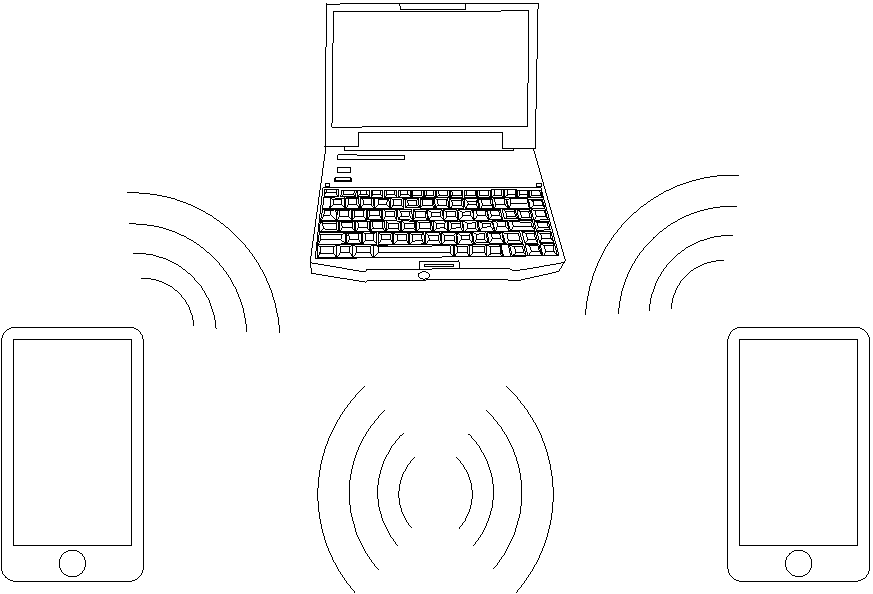
\includegraphics[width=4.5in]{graphs/compucelus.pdf}
    \caption{El diseño de red acústica propuesta puede contener nodos heterogéneos, tales como teléfonos del tipo smartphone o computadoras personales.}
    \label{arch:chain}
\end{figure}

Un canal óptico es un claro ejemplo de canal Z, pero también es posible realizar un canal Z con redes acústicas si se utilizan ciertas modulaciones.

Los enlaces ópticos presentan como mayor desventaja la necesidad de, o bien transmitir los pulsos de luz mediante una fibra óptica entre los nodos comunicantes, o que exista visibilidad directa entre ambos nodos, una condición que no puede ser garantizada en todos los ambientes de trabajo. Además, los sensores ópticos requeridos generalmente no están presentes en los clientes y deben ser instalados separadamente.

Sin embargo, la transmisión sobre un canal acústico tiene como ventaja el poder utilizar hardware instalado en la mayoría de los potenciales clientes, tales como parlantes o micrófonos estándar, elementos comunes en dispositivos electrónicos masivos \cite{citeulike:12800468}. Además, no es necesaria la visibilidad directa mientras ambos nodos estén localizados a pocos metros de distancia.

En contraste con otras tecnologías como RF o enlaces ópticos, la naturaleza del canal acústico y la facilidad para interceptar o registrar comunicaciones utilizando este medio hace de la privacidad un requerimiento esencial. Algunos sistemas de comunicación de audio han sido propuestos \cite{august2002apparatus}, pero el problema de la privacidad en este tipo de comunicaciones se soluciona generalmente en la capa de aplicación, es decir, en alto nivel. Esta Tesis presenta una aproximación a la seguridad y privacidad desde la capa física, basada también en time-hopping CDMA, similar a aquella presentada en \cite{6476559}. Presentaremos una red segura acústica punto a punto y punto a multipunto de corto alcance y bajo consumo, que no requiere de ningún hardware adicional en clientes móviles.

Un escenario válido para la aplicación de esta tecnología podría ser validación de transacciones financieras pequeñas tales como terminales PoS \textit{(Point of Sale)} o cajeros automáticos (ATM) utilizando un dispositivo móvil (por ejemplo, un celular del tipo \textit{smartphone}) sin modificaciones de hardware. Una tecnología similar que se utiliza en estos casos es la denominada NFC \textit{(Near Field Communications)} \cite{nikitin2007overview}, un protocolo inalámbrico que requiere hardware especializado que, al momento presente, no se encuentra disponible en la mayoría de los dispositivos móviles.
Con respecto a la implementación sobre el medio óptico, es necesario ajustar algunos parámetros, como por ejemplo el tamaño de trama, que se reduce de $M=4096$ a $M=256$ para la implementación acústica, y el parámetro $K=9$ que es el óptimo para el $M$ seleccionado. El número de clientes también se ve reducido de $N=128$ a $N=12$ ya que al ser la red acústica de corto alcance, no se prevé una elevada cantidad de clientes simultáneos. En la figura \ref{arch:AudioSimul} se muestra una simulación del sistema con estos parámetros contrastada con una medición realizada entre una Notebook (T420) y un celular (Lenovo A789).  En dicha figura se puede apreciar que las simulaciones y las mediciones son similares, mostrando estas últimas desde 14 clientes en adelante. La razón por la cual sólo se muestra a partir de 14 clientes reside en que la tasa efectiva de transmisión es muy baja y para medir un BER más grande, se necesitaban tiempos del orden de un día. Teniendo en cuenta que este tipo de sistemas se utilizarían para transacciones de pocos bytes, y la coincidencia entre la curva simulada y la real, consideramos que el desempeño es adecuado.

\begin{figure}[t]
  \centering
    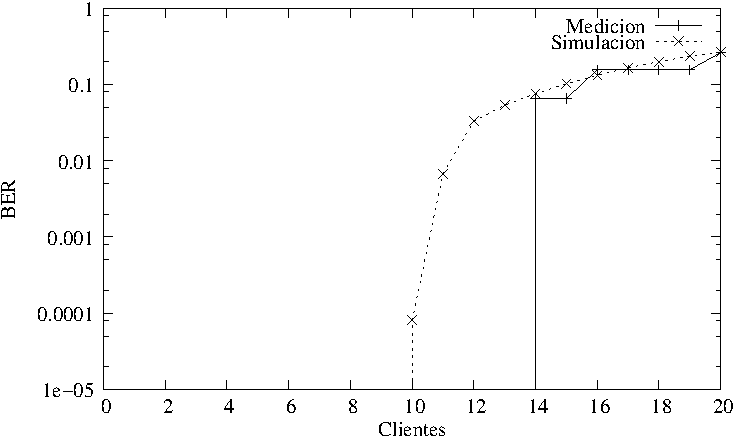
\includegraphics[width=5in]{graphs/audio-fig6}
    \caption{Simulación y medición del BER para una red acústica en función del número de clientes con M=256 y K=9.}
    \label{arch:AudioSimul}
\end{figure}



\subsection{Redes acústicas: arquitectura}

Una ventaja importante del sistema acústico propuesto es su simplicidad, requiriendo solamente un emisor de sonido (parlante), un receptor (micrófono) y un canal de transmisión de sonido que puede ser aire (y, en casos más especializados, agua). Ambos requerimientos están generalmente disponibles en computadoras, notebooks, tablets y teléfonos celulares. 
El esquema lógico es el mismo que el descrito anteriormente: time-hopping CDMA seguro, códigos correctores de errores y un método de sincronización a nivel de bit.
Como resultado, el sistema soporta canales unidireccionales a los clientes que sirven tanto para comunicaciones punto a punto como punto a multipunto. 
Para la implementación de canales bidireccionales, pueden utilizarse dos canales separados (ej. utilizando dos códigos CDMA diferentes), o empleando el mismo canal de manera \textit{half duplex}, aunque este último modo de funcionamiento necesita de desarrollo adicional y no es el objetivo de esta Tesis.
En las próximas secciones se describe el sistema en mayor detalle.

\subsection{Redes acústicas: modulación y sincronización}
\begin{figure}[t]
  \centering
    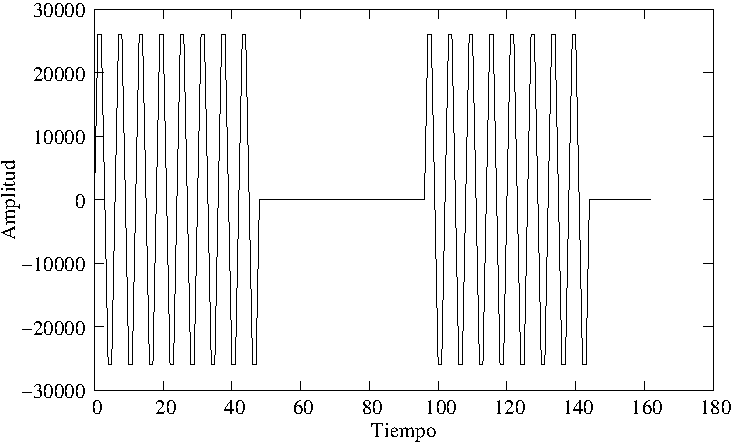
\includegraphics[width=5in]{graphs/modulated.pdf}
    \caption{Modulación OOK.}
    \label{arch:ook}
\end{figure}


A diferencia de la implementación óptica donde se utilizaron algunas funciones provistas por el hardware de FPGA, tales como el mecanismo de sincronización de bit, para la transmisión acústica se implementaron tanto el algoritmo de modulación como el de sincronización totalmente en software.
Para la modulación, fue utilizado el algoritmo de OOK (ver figura \ref{arch:ook}), que codifica los bits a transmitir como pulsos. La frecuencia de portadora puede variar de 10 kHz a 16 kHz, y la tasa de transmisión se fijo a 1000 bps. Debido a la baja velocidad de este canal se introduce un problema inexistente en la implementación óptica: el retraso de la red (el tiempo que tarda un bit en atravesar toda la red) es alto, debido principalmente a la etapa de Reed-Solomon que necesita recibir 256 bytes para comenzar el proceso de decodificación del bloque. Debido a que el canal soporta una velocidad máxima de 1000 bps, el retraso puede alcanzar niveles inaceptables, del orden de los 30 segundos.
Una selección mas apropiada del algoritmo de FEC (tal como BCH) podría reducir reducir el retraso total del sistema.
Adicionalmente, una etapa de \textit{pulse shaping} o formación de pulso fue implementada, utilizando un filtro pasa-banda a la salida de la modulación y también en la entrada del demodulador. Este filtro ayuda a rechazar interferencia acústica o ruido ambiente.

\begin{figure}[t]
  \centering
    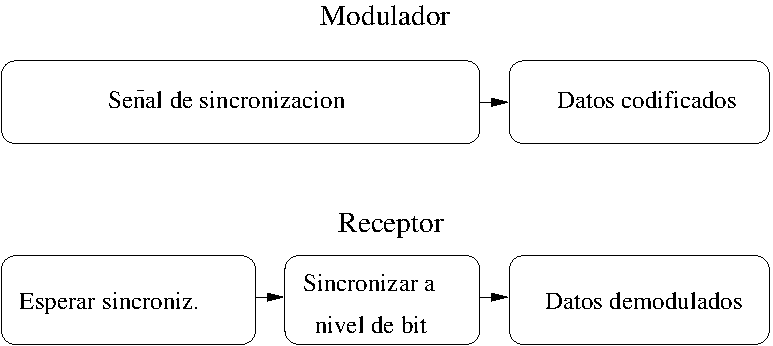
\includegraphics[width=4.5in]{graphs/Audio-Sync2.pdf}
    \caption{Sincronización.}
    \label{arch:sync}
\end{figure}


La sincronización entre un transmisor y un receptor es esencial para la decodificación correcta de la información. Por esta razón, un patrón de sincronización inicial es enviado, para que el receptor pueda ajustar parámetros tales como la fase y nivel de decisión de la señal (ver figura \ref{arch:sync}). La deriva \textit{(drift)} del reloj y variabilidad \textit{(jitter)} no son significativas a esta baja velocidad de transmisión y ninguna corrección en tiempo real es requerida, por lo que la implementación del módem por software es simple.
El nivel de decisión del demodulador es dinámico, es decir que es constantemente recalculado utilizando los niveles de entrada promediados.
La fase del símbolo recibido también es corregida utilizando los mismos datos de entrada como referencia.

